\section{Algorithm Implementation}

This section will provide an outline to the implementation of both of the fuzzy entropy algorithms including the fuzzy-set membership implementation and a brief outline of the Shannon entropy implementation provided in the demo code by Learned-Miller \cite{joint-alignment}.

More information on the new functions created for this project, along with functions modified and utilised from the existing code base can be found in Appendix \ref{appendix:code}.

\subsection{Membership Implementation}
\label{ssec:member-imp}

As covered in Section \ref{sssec:member}, the Membership trapezia would be defined within the system, rather than dynamically being calculated. This made use of the Fuzzy Logic Toolbox \cite{fuzzy_toolbox} by leveraging the following functions:

\begin{itemize}
  \item \textbf{trapmf: } trapezium-shaped membership function
  \item \textbf{evalmf: } a generic membership evaluation function
\end{itemize}

Having pre-defined functions for creating and evaluating the membership trapezia ensured that the function was a quick implementation. However it did reduce the number of Unit Tests that could be written to test the creation of such elements.

In this function, an image is read in, the membership of each pixel is evaluated against each of the two or three membership trapezia, adding the outcome to a corresponding array (e.g. one array for the membership of all the pixels against the low-trapezium etc). The two or three arrays (depending on the number of trapezia) are then compared and the element at position $x$,$y$ with the greatest membership value is added to another array which collates all of the highest values.

For example:

\begin{minted}
  [
  breaklines,
  frame=lines,
  framesep=2mm,
  baselinestretch=1.2,
  fontsize=\small,
  linenos
  ]
  {text}
    pixel[1,1]`s membership in trapezium low = 0.8
    pixel[1,1]`s membership in trapezium medium = 0.4
    pixel[1,1]`s membership in trapezium high = 0

    Therefore as 0.8 is the highest membership value, this is added to the image membership array
\end{minted}

The three/four arrays (one for each trapezium and one for the highest values) are then passed out of the function, and utilised in both of the fuzzy entropy algorithm functions.

\newpage
\subsection{Shannon Entropy}
\label{ssec:shannon-entropy}

Learned-Miller's demo code came with an implementation of Shannon Entropy \cite{joint-alignment}. Whilst originally the predominant dataset was MNIST handwriting data \cite{lecun1998gradientbased}, which is a binary dataset (pixels were either black or white), this was not useful for this project as there is no variation in greyscale, even when a mean is taken of multiple images.

However, Learned-Miller had included extra code to handle the processing of greyscale and colour images, such as in MRI images. This ensured that no function needed to be created to handle greyscale images, greatly reducing the pre-programming needed. The only image handling that was encountered was to do with the mammograms, and the creation of a large pgm file to pass into the \Gls{Congealing} algorithm.

As outlined in \ref{ssec:entropy}, Shannon entropy is defined as:

\begin{equation}
  H(X) = - \displaystyle\sum_{i=0}^{N}{p_i \log_2 p_i}
\end{equation}

\subsubsection{MATLAB implementation}

This can be computed very quickly using a lookup table containing all the possible values of $p$. This makes it likely that the Shannon entropy algorithm will be the quickest on each iteration. However as it does not take any type of uncertainty into consideration when aligning the scans, the outcome could be quite dramatically different from that of a Fuzzy entropy nature.

Learned-Miller's Shannon entropy implementation has been retained, and can be found in the function \texttt{fastEntLookup.m} which is how it was originally named. Where possible, when original functions have been used, their original file names have been kept the same.

The function itself needed no changes to fit in with this project, however the way in which it is called by both \texttt{binaryCongeal.m} and \texttt{incrTrans.m} has been adapted so the user can choose which alignment metric to use when congealing their images.

\newpage
\subsection{Non-Probabilistic Entropy}
\label{ssec:non-prob-sec}

As outlined in Section \ref{sssec:non-prob-review}, De Luca \& Termini`s Non-Probabilistic entropy can be defined as:

\begin{equation}
  \label{eq:de-luca}
  H_A = -K \displaystyle\sum_{i=1}^{n}{\{\mu_i\log(\mu_i) + (1 - \mu_i)\log(1 - \mu_i)\}}
\end{equation}

%Al-sharhan et al's paper compiling several Fuzzy Entropy algorithms \cite{Al-Sharhan_Karray_Gueaieb_Basir_2001} contains a methodical,in-depth derivation of their algorithm, and has been instrumental in building my knowledge on the algorithm in question.

We will assume $-K$, the positive constant, is defined as $\frac{1}{n}$ as outlined in \cite{DeLuca_Termini_1972}.

%==============================================================================
\subsubsection{MATLAB implementation}
%==============================================================================

After some research into current implementations of Fuzzy Entropy algorithms in MATLAB, it was concluded the best approach would be to implement De-Luca \& Termini's algorithm from scratch. This entailed creating a membership function, which computes the grey-level membership of each pixel in the mean image (calculated from a set of input images).

This array of pixel memberships is fed into a \texttt{nonProbabilistic.m} function where it is iteratively passed into latter part of equation \ref{eq:de-luca} \big(after $\displaystyle\sum$\big). The output array is then summed and multiplied by $\frac{1}{n}$ as defined in Equation \ref{eq:de-luca} and Subsection \ref{sssec:non-prob-review}. The final mean pixel entropy is calculated by taking the image entropy and dividing by the number of pixels in the image.


%==============================================================================
\subsubsection{Technical challenges}
%==============================================================================

The main technical challenge for this implementation is ensuring maximum optimisation to keep running times to a minimum. Leveraging MATLAB's own Toolbox for calculating the membership saves a lot of time and lines of code, however it was important to check what they call from within. One membership function was redrawing the trapezia every time it was called, significantly slowing down the process - reducing the amount of times the initial function was called helped reduced the run-time by over 60seconds. This challenge of optimisation is covered in-depth in the latter Subsection \ref{ssec:vectorisation}.

\newpage
\subsection{Hybrid Entropy}
\label{ssec:hybrid-sec}

As mentioned in Section \ref{sssec:hybrid-section}, the Hybrid Entropy equation is as follows:

\begin{equation}
  H_{hy} = -p_0\log(1 - E_0) - p_1\log(E_1)
\end{equation}

Where $E_0$ and $E_1$ can be defined as:

\begin{subequations} %\label{eq:E0-E1}
  \begin{align}
    &E_0 = \frac{1}{n}\displaystyle\sum_{i=1}^{n}{(1-\mu_i)exp(\mu_i)} \\
    &E_1 = \frac{1}{n}\displaystyle\sum_{i=1}^{n}{\mu_iexp(1-\mu_i)}
  \end{align}
\end{subequations}

And $p_0$ and $p_1$ are the probabilities of receiving 0 and 1 symbols respectively.

%==============================================================================
\subsubsection{MATLAB implementation}
%==============================================================================

Due to reasons covered in Subsection \ref{sssec:hyrid-technical}, Hybrid Entropy membership was implemented using 2 trapezia covering 2 fuzzy sets, as seen in Figure \ref{fig:2-traps}.

\begin{figure}[H]
  \center
  \includegraphics[scale=0.4]{Chapter2/hybrid-img/2_traps.png}
  \caption{Two membership trapezia for Hybrid Entropy - Low and High grey-level values.}
  \label{fig:2-traps}
\end{figure}

Two arrays are then fed into the Hybrid Entropy function - one listing all the pixel membership values from the low trapezium, and the other from the high trapezium. The final entropy is taken as a comparison between the low and high fuzzy sets.

%==============================================================================
\subsubsection{Technical challenges}
\label{sssec:hyrid-technical}
%==============================================================================

Whilst Hybrid Entropy utilises a membership function, much like Non-Probabilistic entropy, it was derived to work with binary entropy, not the ternary membership modeled for Non-Probabilistic. Because of the binary nature, the equation uses `inversion' to depict if not this fuzzy set, then must belong to the other.

Experimentation was done as to whether the equation could be adapted in such a way to continue using three separate membership trapezia - low, medium and high grey-level values. Logic would dictate that if the comparison of two fuzzy sets works, then to compare the low fuzzy set to the medium, the medium to the high and the high to the medium should work.

In theory, calculating $E_0$ and $E_1$ for each trapezium, calculating the hybrid entropy for each, and then combining them, should work:

\begin{equation}
E_0 = \frac{1}{\text{No. of pixels in low trapezium}}\displaystyle\sum_{i=1}^{n}{(1-Low\mu_i)exp(Low\mu_i)}
\end{equation}
\begin{equation}
E_1 = \frac{1}{\text{No. of pixels in low trapezium}}\displaystyle\sum_{i=1}^{n}{Low\mu_iexp(1-Low\mu_i)}
\end{equation}

Where $Low\mu$ is the membership of the pixels in the low fuzzy set.
%http://tex.stackexchange.com/questions/112238/how-to-wrap-a-long-equation-in-latex
\begin{equation}
H_{hy} = -p_0\log_{10}(1 - E_0) - p_1\log_{10}(E_1)
\end{equation}

Where

$p_0 = \frac{\text{No. of pixels in low trapezium}}{\text{No. of pixels in low trapezium + med trapezium}}$

and

$p_1 = \frac{\text{No. of pixels in med trapezium}}{\text{No. of pixels in low trapezium + med trapezium}}$


This was done for all 3 trapezia, then combined and divided by 3 (for the mean entropy). As the result for each trapezium should be between 0 and 1 (as each is an entropy value), then combining them should be no issue. However this was not the case.

First of all, the hybrid equation output was deemed to be `NaN' - something which generally occurs when attempting to divide by 0. Anomalous outputs from the high trapezium was to be expected, as there are very few pixels which fall within the range nearer the white end of the grey-level scale. This was mitigated by setting any `Nan' output equal to 0, in effect ignoring that particular output from the highest fuzzy set.

After this mitigation, the third and fourth iteration had suitable entropy values, however the fifth entropy value was a negative, something which is not possible in terms of entropy, as it must be between 0 and 1 - see Figure \ref{fig:minus-entropy}.

\begin{figure}[H]
  \begin{center}
    \pgfplotsset{every axis/.append style={thick},width=0.4*\textwidth, ymax=1}
      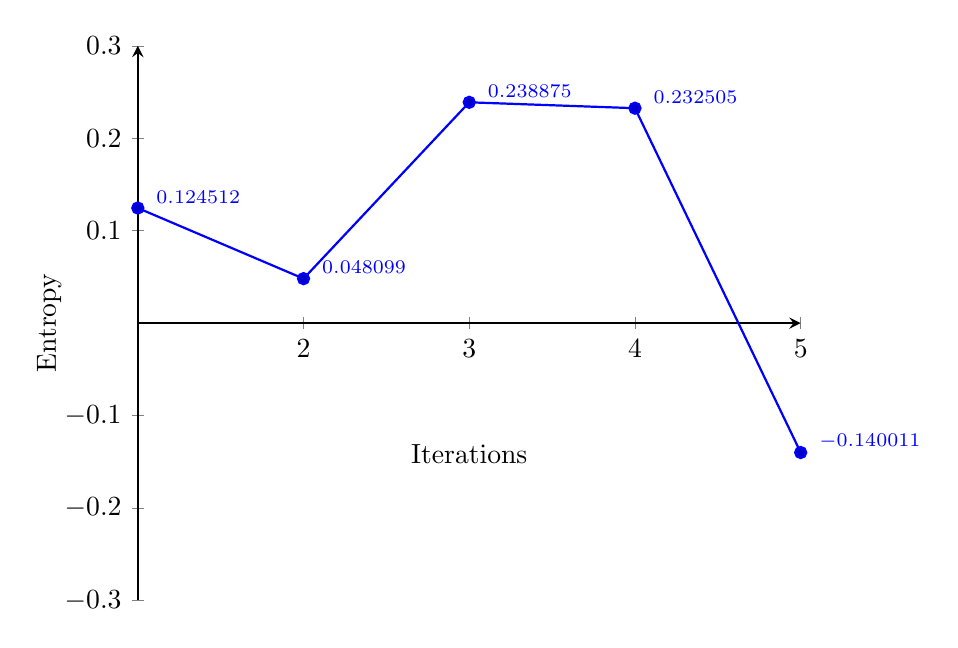
\begin{tikzpicture}
        \begin{axis}[
          width = 10cm,
          axis lines = middle,
          xlabel = {Iterations},
          ylabel = {Entropy},
          ymin = -0.3,
          ymax = 0.3,
          ytick={-0.5,-0.4,...,0.6},
          y tick label style={
                 /pgf/number format/.cd,
                  fixed,
                  fixed zerofill,
                  precision=1,
              /tikz/.cd
          },
          xtick={1,2,...,5},
          x label style={at={(axis description cs:0.5,0.3)},anchor=north},
          y label style={at={(axis description cs:-0.1,.5)},rotate=90,anchor=south},
          nodes near coords,
      	  nodes near coords align={vertical},
          every node near coord/.append style={font=\scriptsize,
                  xshift = +3pt, yshift=+4pt,anchor=west, /pgf/number format/precision=6},
          ]
        \addplot coordinates
          { (1, 0.124512) (2, 0.048099) (3, 0.238875) (4, 0.232505) (5, -0.140011) };
          \draw[ultra thin] (axis cs:0,\pgfkeysvalueof{/pgfplots/ymin}) -- (axis cs:0,\pgfkeysvalueof{/pgfplots/ymax});
        \end{axis}
      \end{tikzpicture}
    \end{center}
    \caption{Graph showing the entropy output after 5 iterations}
    \label{fig:minus-entropy}
\end{figure}

It was concluded that the implementation of three fuzzy sets within Hybrid Entropy would not be realistic within the remaining time-frame of the project, and the membership for Hybrid Entropy was redefined to the concept of 2 fuzzy sets, as derived by Pal and Pal. This would mean one trapezium for pixel grey-level values with low values, overlapping with a high grey-level value trapezium at approximately 128, as seen in Figure \ref{fig:2-traps}.
